\documentclass{article}
\usepackage{pgfplots}
\usepackage{siunitx}
\usepackage[paperheight=2.9in,paperwidth=3.9in,margin=0in]{geometry}
\pgfplotsset{compat=newest}
\usepgfplotslibrary{external}
\usetikzlibrary{patterns}


\tikzexternalize



\definecolor{pastelred}{rgb}{1.0, 0.41, 0.38}
\definecolor{pastelmagenta}{rgb}{0.96, 0.6, 0.76}\definecolor{pastelpink}{rgb}{1.0, 0.82, 0.86}

\begin{document}
\pgfplotsset{
    every axis plot/.append style={line width=1pt, font=\large,}
}
 \pagenumbering{gobble} 

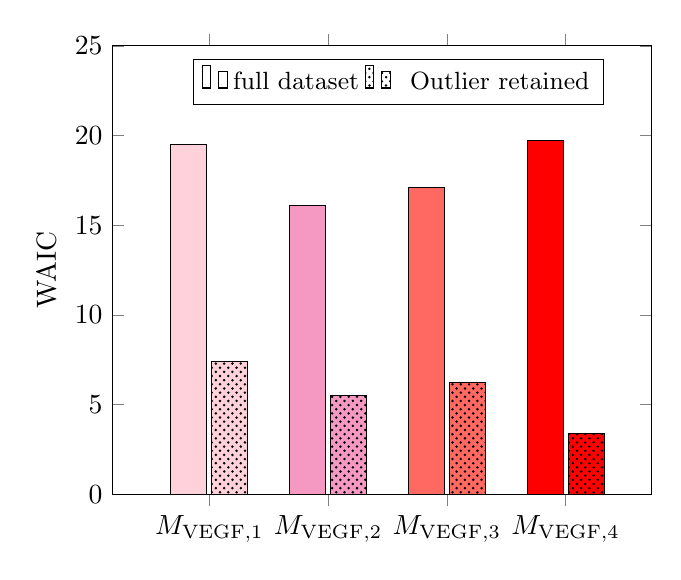
\begin{tikzpicture}
    \begin{axis}[
        ybar,
        ylabel = {WAIC},
        ymin=0, ymax=25,
        xmin=1,xmax=6,
        bar width=13pt, 
        legend columns=2,
        xtick={-1.3,2,5.3,8.6},
        xticklabels={$M_{\text{VEGF},1}$,$M_{\text{VEGF},2}$,$M_{\text{VEGF},3}$,$M_{\text{VEGF},4}$},
         legend style={/tikz/column 3/.style={column sep=5pt},at={(0.53,0.97)}, anchor=north, font=\small },
        enlarge x limits=1]

        \addplot [ybar, width=30pt, fill=white] plot coordinates {
                (-10, 19.5)
                };
        \addplot [ybar, fill=white, postaction={
        pattern=crosshatch dots
                }] plot coordinates {
                (-10, 7.4)
                }; 
        
        \addplot [ybar, width=30pt, fill=pastelpink] plot coordinates {
                (1, 19.5)
                }; 
        \addplot [ybar, fill=pastelpink, postaction={
        pattern=crosshatch dots
    }] plot coordinates {
                (1, 7.4)
                };  
        \addplot [ybar, fill=pastelmagenta,
] plot coordinates {
                (2, 16.1)
                }; 
        \addplot [ybar, fill=pastelmagenta, postaction={
        pattern=crosshatch dots
    }] plot coordinates {
                (2, 5.5)
                }; 
                
       \addplot [ybar, fill=pastelred,
] plot coordinates {
                (3., 17.1)
                }; 
        \addplot [ybar, fill=pastelred, postaction={
        pattern=crosshatch dots
    }] plot coordinates {
                (3., 6.23)
                }; 

       \addplot [ybar, fill=red,
] plot coordinates {
                (4., 19.7)
                }; 
        \addplot [ybar, fill=red, postaction={
        pattern=crosshatch dots
    }] plot coordinates {
                (4., 3.4)
                };   

     \legend{full dataset, Outlier retained}   
     
     \end{axis}
\end{tikzpicture}
\end{document}               

        


